\documentclass[12pt,xcolor=table]{beamer} 
\usepackage{beamerthemesplit}
\usepackage{beamerthemeshadow}

\definecolor{blue}{rgb}{0, 0, 0.25}
\setbeamertemplate{navigation symbols}{} 
\setbeamertemplate{headline}{}
\definecolor{blue}{rgb}{0, 0, 0.25}
\setbeamercolor{structure}{fg=blue}

\usepackage{caption}
\captionsetup{font=scriptsize,labelfont=scriptsize}
\setbeamerfont{caption name}{series=\bfseries}
\setbeamerfont{section in toc}{size=\large}
\setbeamerfont{subsection in toc}{size=\small}
\setbeamertemplate{caption}[numbered]

\usepackage{verbatim}
\newenvironment{colorverbatim}[1][]%
{%
\color{black}
}%

\usepackage{mathpazo,courier,euler}
\usepackage{listings}

\lstset{language=sh,
    basicstyle=\ttfamily\bfseries,
    showstringspaces=false,
    keywordstyle=\color{black}\bfseries}

\logo
{
\hspace{270pt}

\includegraphics[scale=0.17]{images/iitb-logo.png}
}

\setbeamercolor{structure}{fg=blue}
\setbeamercolor{alerted text}{fg=blue}
%\beamertemplateshadingbackground{blue!20}{white!20}
\usepackage{listings}
\setbeamertemplate{frametitle continuation}[from second]
\addtobeamertemplate{navigation symbols}{}{%
    \usebeamerfont{footline}%
    \usebeamercolor[fg]{footline}%
    \hspace{1em}%
    \insertframenumber/\inserttotalframenumber
}
\usepackage{multirow}
\usepackage{graphicx}
\usepackage{hyperref}
\usepackage[backend=biber,sorting=none]{biblatex}
\addbibresource{mybibliography.bib}

\title[Edge following using Kilobots]{Edge following using Kilobots}
%\subtitle{A finite state machine approach}
 
\author[Abhishek, Harsha Priyanka, Neelam]{Abhishek\inst{1} \and Harsha Priyanka\inst{1} \and Neelam\inst{1}}
 
\institute[IIT Bombay] % (optional)
{
  \inst{1}%
  M.Tech scholar\\
  Systems and Control Engineering
}

\date[] 
{\href{http://www.iitb.ac.in/}{Indian Institute of Technology, Bombay}\\\today}


\begin{document}

\begin{frame}
   \titlepage
\end{frame}

\AtBeginSection[]
{
	\begin{frame}<beamer>
	\frametitle{Overview}
	\tableofcontents[currentsection]
	\end{frame}
}


\begin{frame}{Overview}
\tableofcontents
\end{frame}
\section{Introduction}
\begin{frame}
	\frametitle{Kilobots}
	\begin{columns}		
		\begin{column}{0.5\textwidth}
			\textbf{Specifications}
			\vspace{0.2cm}
			\begin{itemize}
				\item ATmega 328p processor 
				\item Li-Ion 3.7V battery 
				\item One IR transmitter-receiver pair 
				\item One light sensor 
				\item Two vibration motors (1 cm/sec, 45 degrees/sec)
			\end{itemize}
		\end{column}
	\begin{column}{0.5\textwidth}
		\begin{figure}
			\centering
			\fbox{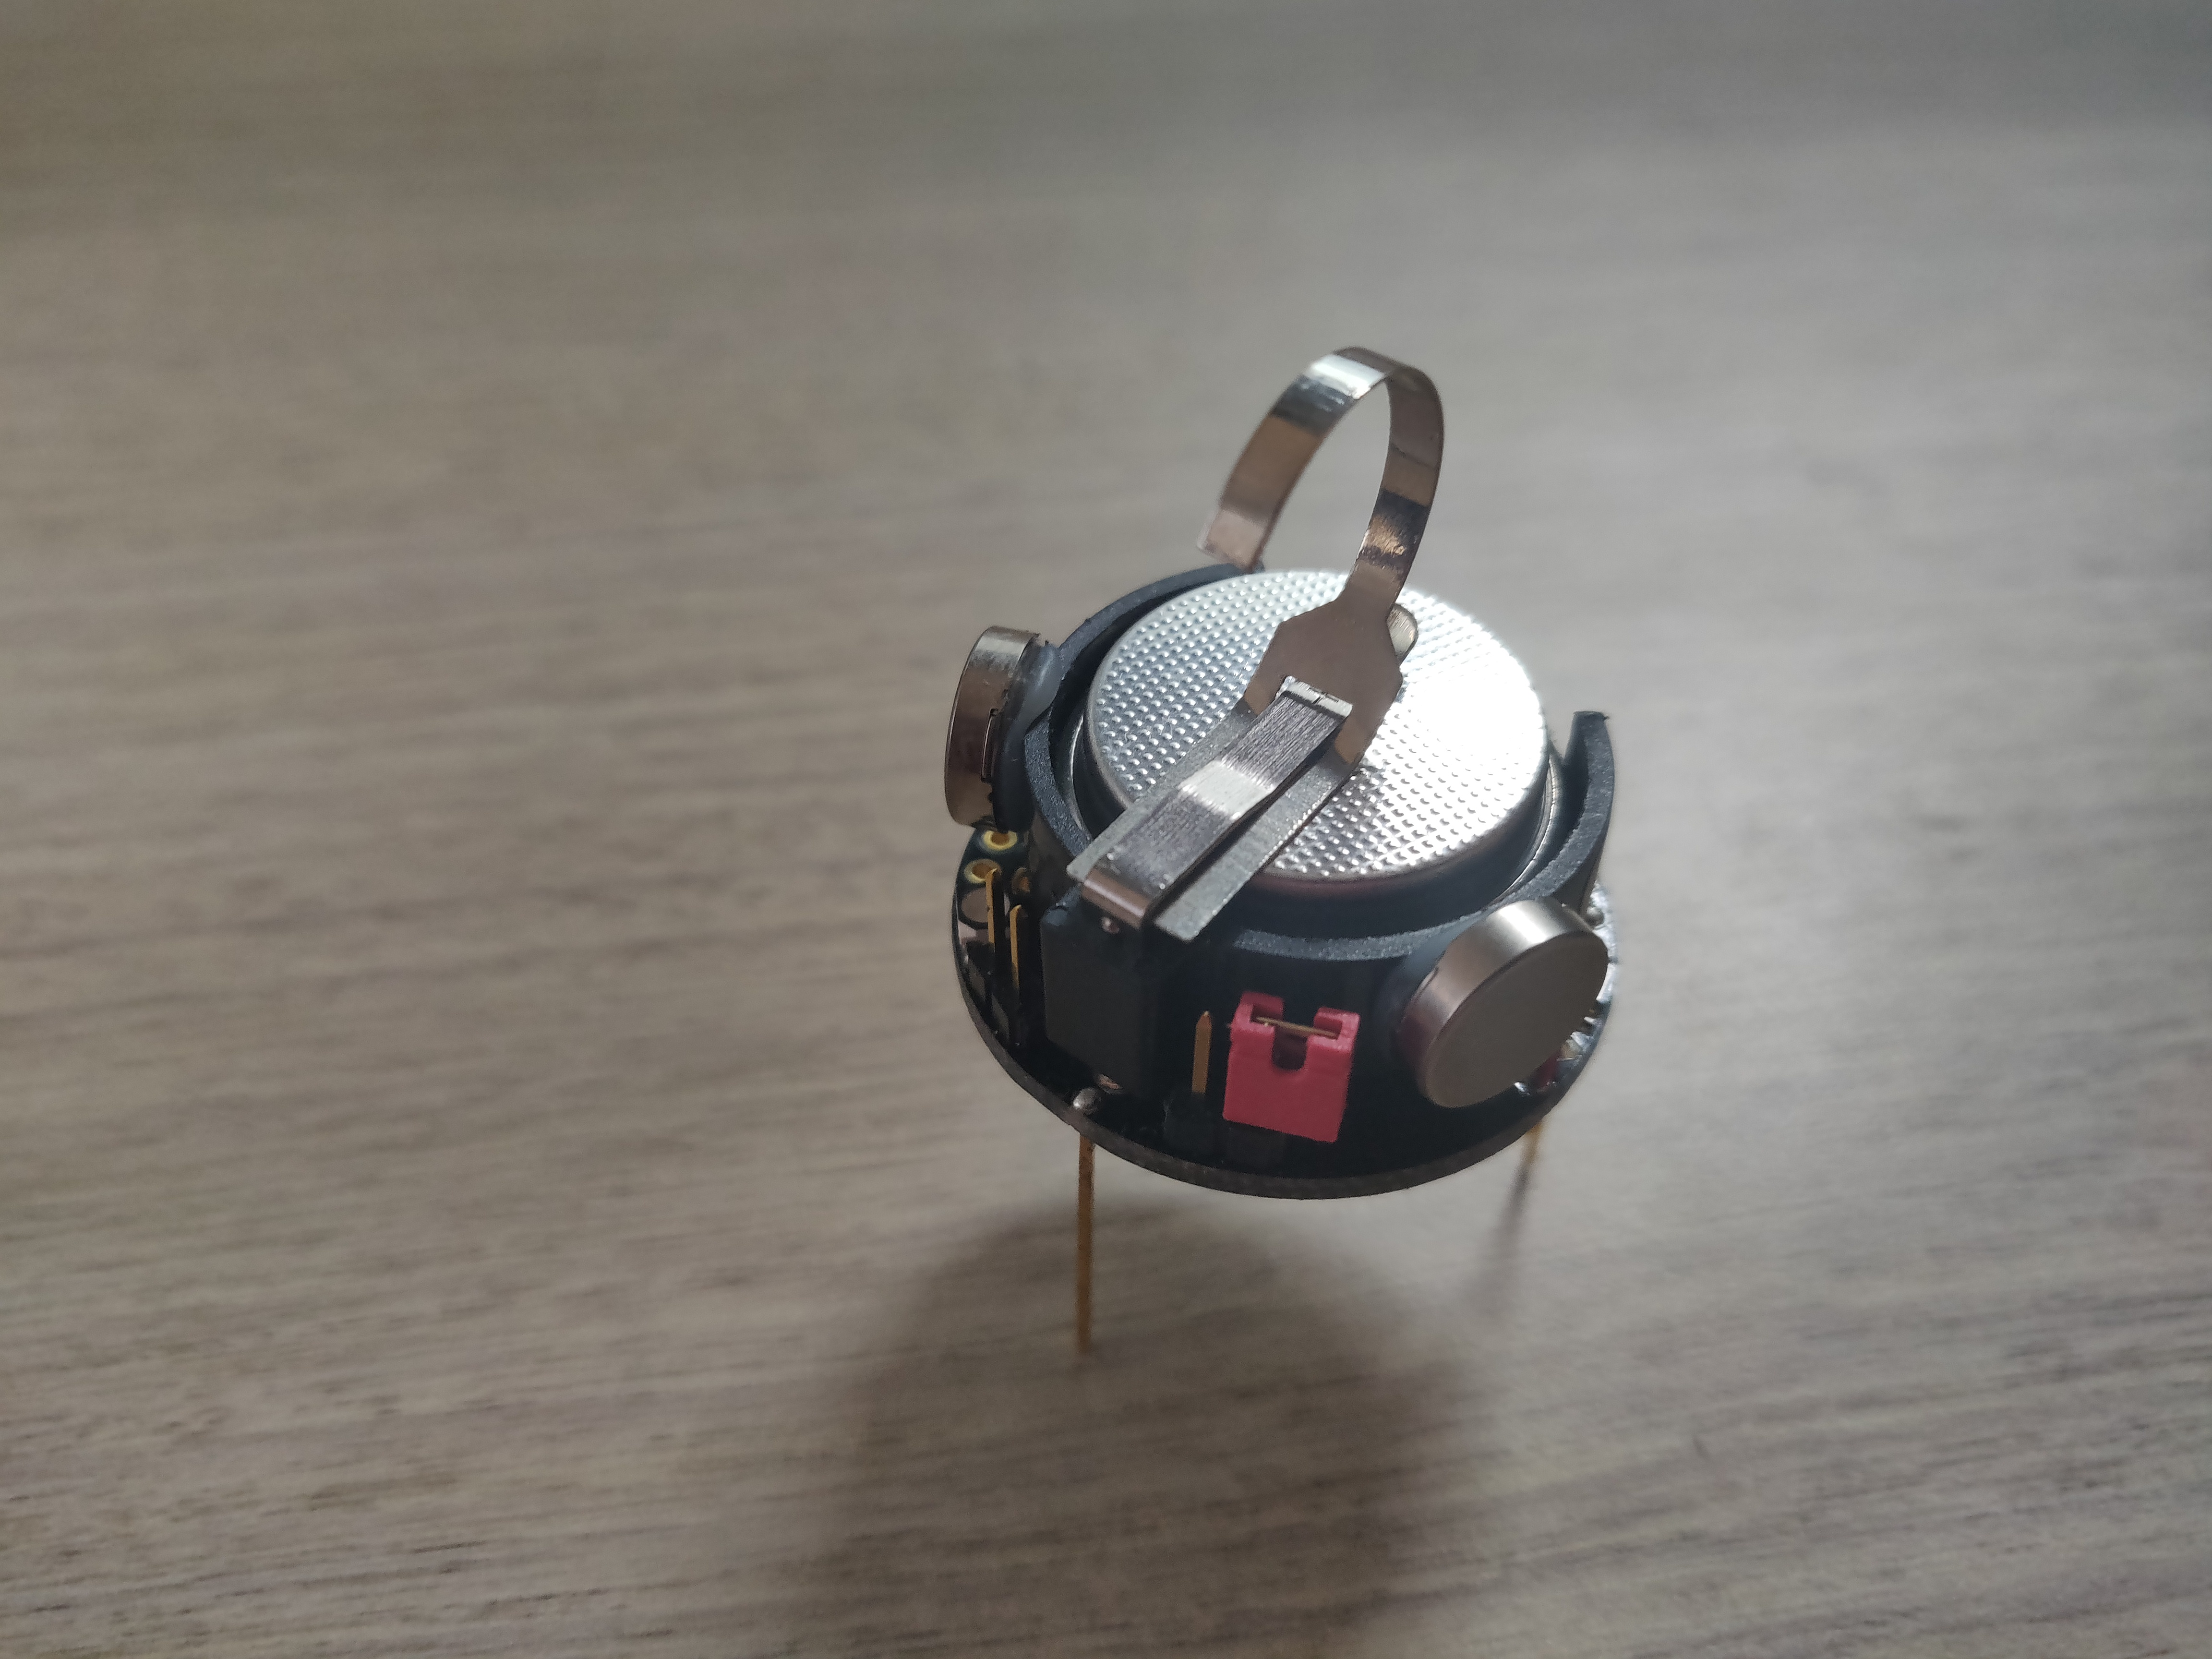
\includegraphics[scale=0.03]{images/kilobot.jpg}}
			\vspace{0.2cm}
			\caption{Kilobot}
		\end{figure}
	\end{column}
	\end{columns}
\end{frame}

\begin{frame}
	\frametitle{About Kilobots \cite{kilobotics_manual}}
	\begin{columns}
		\begin{column}{0.5\textwidth}
			\begin{figure}
				\centering
				\fbox{\includegraphics[scale=0.03]{images/IR-communication.jpg}}
				\vspace{0.2cm}
				\caption{Communication between two Kilobots}
			\end{figure}
		\end{column}
		\begin{column}{0.5\textwidth}
			\begin{itemize}
				\item Reflecting IR light
				\item Communication up to 7 cm (32kb/s) away 
				\item Using over-head controller(OHC)
			\end{itemize}
		\end{column}
	\end{columns}
\end{frame}

\begin{frame}
	\frametitle{KiloGUI}
	\begin{itemize}
		\item Upload new programs 
		\item Motor calibration of the robots    
		\item Set unique ID manually
	\end{itemize}
\end{frame}

\begin{frame}
	\frametitle{KiloGUI}
	\begin{columns}[b]
	\begin{column}{0.5\textwidth}
		\begin{figure}
			\centering
			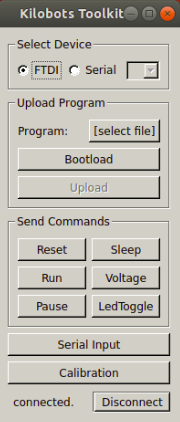
\includegraphics[scale=0.35]{images/kilogui.png}
			\vspace{0.2cm}
			\caption{KiloGUI}
		\end{figure}
	\end{column}
	\begin{column}{0.5\textwidth}	
		\begin{figure}
			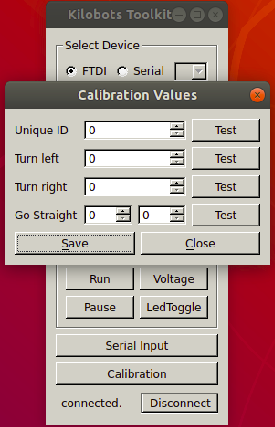
\includegraphics[scale=0.35]{images/kilogui-motor-calib.png}
			\vspace{0.2cm}
			\caption{Motor Calibration}
		\end{figure}
	\end{column}
\end{columns}
\end{frame}

\begin{frame}{Abstract}
\begin{itemize}
    \item Algorithm for self-assembly in Kilobots.
    \item According to \cite{MR-AC-RN:2014}, self-assembly algorithm composes three primitive collective behaviors 
    \begin{itemize}
        \item Edge-following
        \item Gradient Formation
        \item Localization 
    \end{itemize}
    
\end{itemize}
\end{frame}

\begin{frame}{Previous and Present work}
\textbf{Previous work}
\begin{itemize}
    \item Localization
\end{itemize}
\textbf{Present work}
\begin{itemize}
    \item Gradient formation
    \item Edge-following
\end{itemize}

\end{frame}


\section{Orbiting}
\begin{frame}
	\frametitle{Orbiting}
		\textbf{Objective:} Algorithm to allow a planet to orbit around \textit{n} stars from any initial condition.
		\begin{itemize}
		\only<1->{
			\item \textbf{Stars:} Stationary bots around which planet rotates.
			\only<2->{
			\item \textbf{Planet:} Dynamic bots rotating around stars.
			}
		}
	\end{itemize}
\end{frame}

\begin{frame}
\frametitle{With single star}
\framesubtitle{Flowchart}
\begin{figure}[H]
	\centering
	\fbox{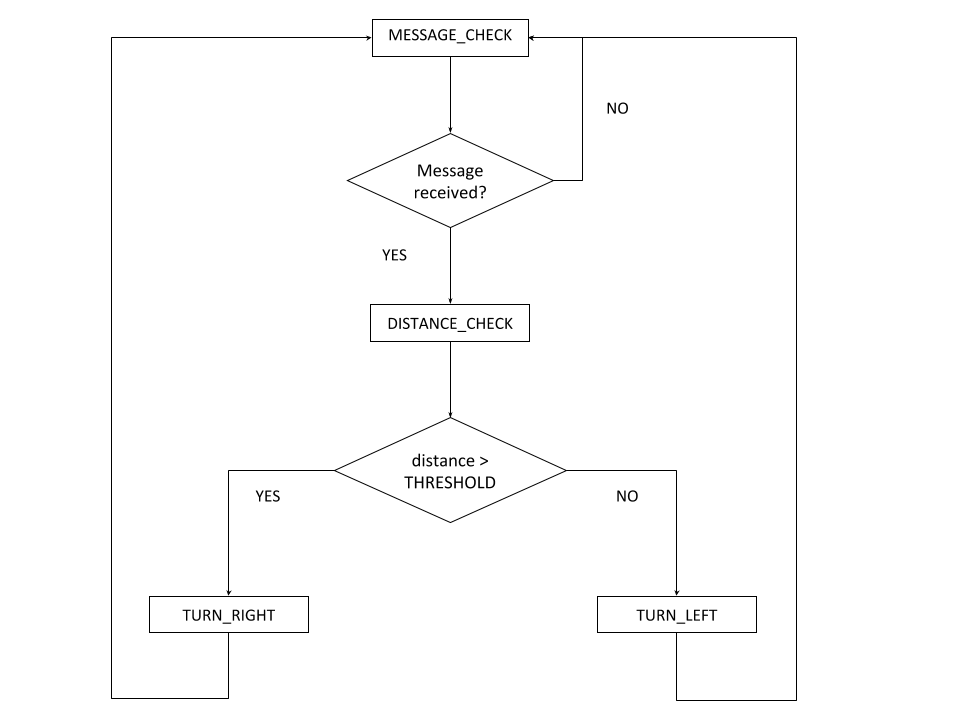
\includegraphics[width=3.6in]{images/flowchart-planet-star.png}}
	\caption{Flowchart for orbiting a Kilobot(Single star)}
	\label{fig:Flowchart_for_orbiting_a_Kilobot(Single_star)}
\end{figure}
\end{frame}

\begin{frame}
\frametitle{With single star}
\framesubtitle{Demonstration}
\begin{figure}[H]
	\centering
	\fbox{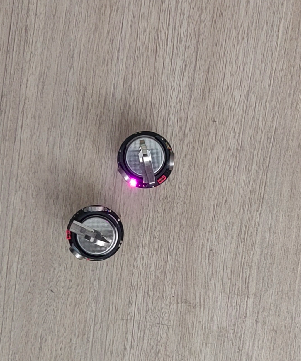
\includegraphics[width=2.0in]{images/planet-star-demo.png}}
	\caption{\href{https://drive.google.com/file/d/1fLfsFgo0ob07vIyrgzMQ1_RKYdbQMO9P/view}{Orbiting of Kilobot (Single Star)}}
	\label{fig:planet-star-demo}
\end{figure}
\end{frame}

\begin{frame}
\frametitle{With multiple stars}
\framesubtitle{Planet-Star Collision Demonstration}
\begin{figure}[H]
	\centering
	\fbox{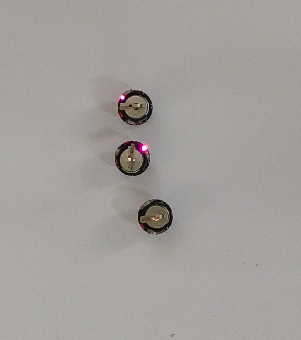
\includegraphics[width=2.0in]{images/planet-mstar-demo.png}}
	\caption{\href{https://drive.google.com/file/d/1OaW0ApBvJGrLmHM_Za6CWgqYbgkAapjx/view}{Planet colliding with one of the stars}}
	\label{fig:planet-star-collision}
\end{figure}
\end{frame}

\begin{frame}
\frametitle{With multiple stars}
\framesubtitle{Escaping the close region}
\textbf{Objective:} Designing a robust algorithm to reach the desired orbit distance without hitting the star.
\end{frame}

\begin{frame}
\frametitle{With multiple stars}
\framesubtitle{Flowchart}
\begin{figure}[H]
	\centering
	\fbox{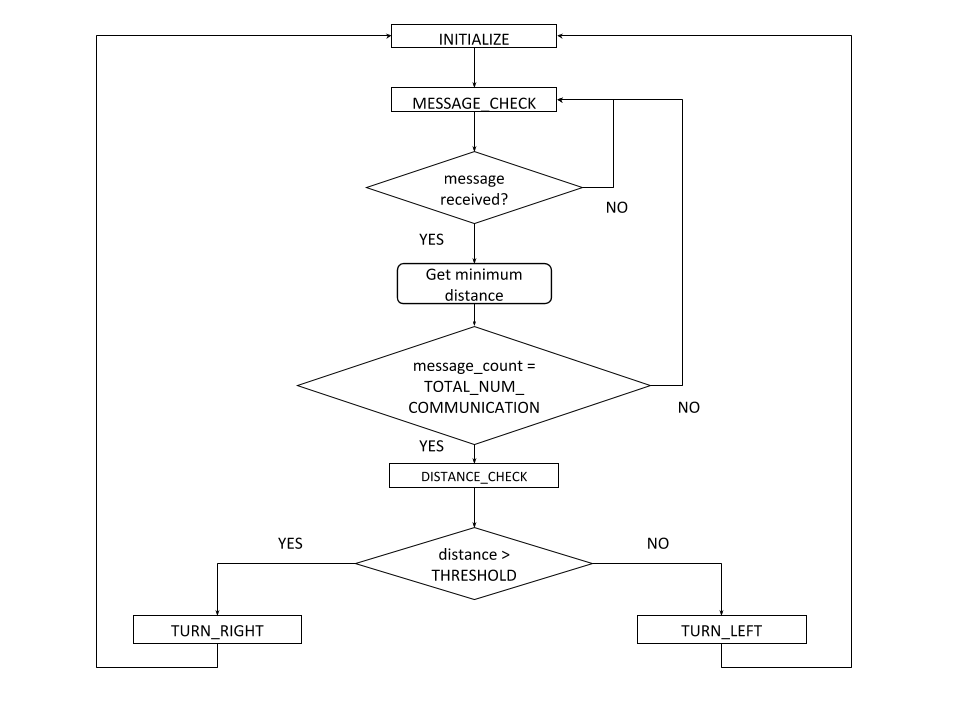
\includegraphics[width=3.5in]{images/flowchart-planet-mstar.png}}
	\caption{Flowchart for orbiting a Kilobot(Multiple star)}
	\label{fig:Flowchart_for_orbiting_a_Kilobot(Multiple_star)}
\end{figure}
\end{frame}

\begin{frame}
\frametitle{With multiple stars}
\framesubtitle{Demonstration}
\begin{columns}[b]
	\begin{column}{0.5\textwidth}
		\begin{figure}[H]
        	\centering
        	\fbox{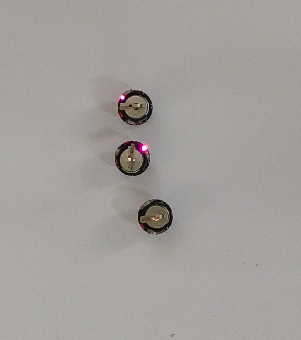
\includegraphics[width=1.3in]{images/planet-mstar-demo.png}}
        	\caption{\href{https://drive.google.com/file/d/1L9QUJOXNgUptjlVbOFi7709xdnPbLLnf/view}{Orbiting of Kilobot (Multiple Star, {\it MOTOR\_ON\_DURATION = 500}, {\it TOTAL\_NUM\_COMMUNICATION = 4})}}
        	\label{fig:planet-mstar-demo-1}
        \end{figure}
	\end{column}
	\begin{column}{0.5\textwidth}	
		\begin{figure}[H]
        	\centering
        	\fbox{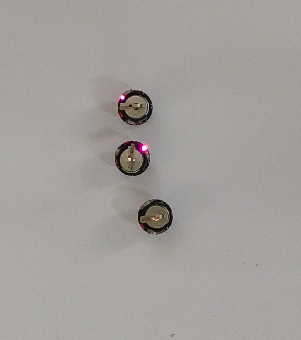
\includegraphics[width=1.3in]{images/planet-mstar-demo.png}}
        	\caption{\href{https://drive.google.com/file/d/1uEPULMZj-hb8SObypaLxKwzrtphcz_XN/view}{Orbiting of Kilobot (Multiple Star, {\it MOTOR\_ON\_DURATION = 800}, {\it TOTAL\_NUM\_COMMUNICATION = 3})}}
        	\label{fig:planet-mstar-demo-2}
        \end{figure}
	\end{column}
\end{columns}
\end{frame}
\section{Gradient Formation}
\begin{frame}
	\frametitle{Gradient Formation}
		\textbf{Objective:} Algorithm to assign unique IDs to Kilobots with respect to a Kilobot using distance as reference.
\end{frame}

\begin{frame}
\frametitle{Flowchart}
\begin{figure}[H]
	\centering
	\fbox{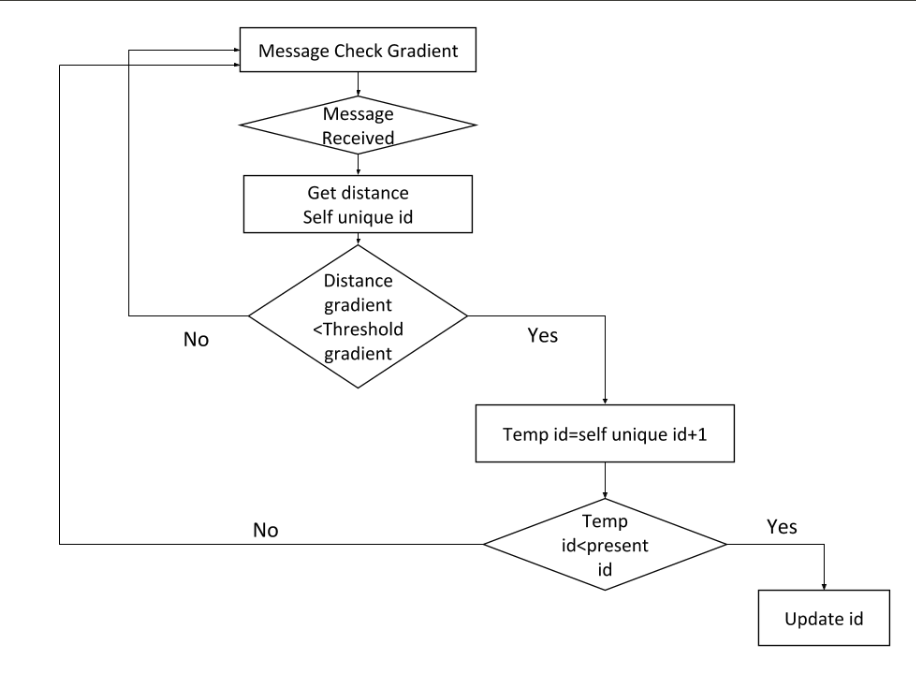
\includegraphics[scale=0.27]{images/flowchart-gradient.png}}
	\caption{Flowchart for gradient formation}
	\label{fig:flowchart-gradient}
\end{figure}
\end{frame}

\begin{frame}
\frametitle{Demonstration}
\begin{figure}[H]
	\centering
	\fbox{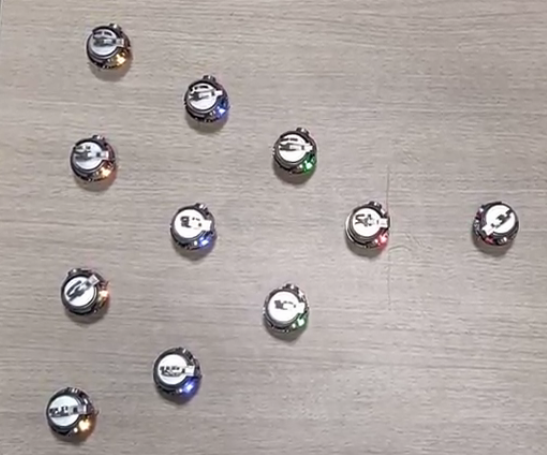
\includegraphics[width=2in]{images/gradient.png}}
	\caption{\href{https://drive.google.com/file/d/1JAcmaJzGgZXJqVzh5EeOXjp7_x3NBJIU/view}{Display of colors as per different ids}}
	\label{fig:gradient-color}
\end{figure}
\end{frame}



\section{Edge Following}
\begin{frame}
	\frametitle{Edge Following}
		\textbf{Objective:} Algorithm to make the kilobots which are on the outer edge to move along the edge of a group of kilobots by measuring distances without being physically blocked and reach the reference bot.
\end{frame}

\begin{frame}
\frametitle{Flowchart}
\begin{figure}[H]
	\centering
	\fbox{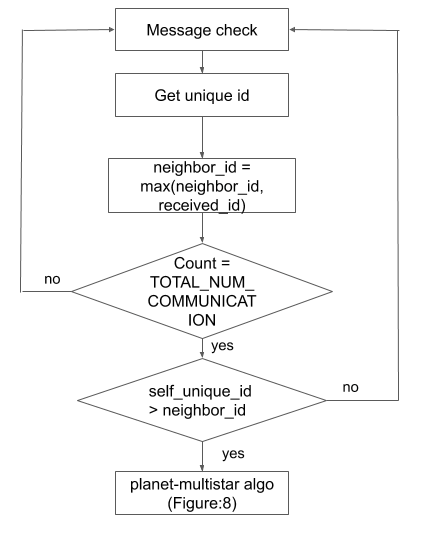
\includegraphics[scale=0.35]{images/flowchart-edge-following.png}}
	\caption{Flowchart for Edge following}
	\label{fig:Flowchart for Edge following}
\end{figure}
\end{frame}

\begin{frame}
\frametitle{Demonstration}
\begin{figure}[H]
	\centering
	    \fbox{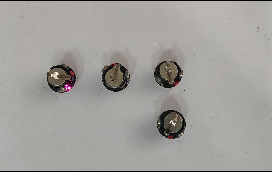
\includegraphics[width=2.5in]{images/edge-following.png}}
	    \caption{\href{https://drive.google.com/file/d/1g10OzQKxJeDGPPiBOiKoj_39G7-d5FFN/view}{Edge Following with \textit{TOTAL\_NUM\_COMMUNICATION=5} and \textit{TOTAL\_NUM\_COMMUNICATION\_ORBIT=3}}}
	    \label{fig:Edge Following}
\end{figure}
\end{frame}



\section{Gradient and Edge Following Integration}
\begin{frame}
	\frametitle{Edge Following}
		\textbf{Objective:} Algorithm to form  gradient  with  respect  to  reference  robot  first  and then bring the farthest robot near the reference robot by using edge following algorithm.  We are integrating the gradient formation and edge following experiments performed earlier.
\end{frame}

\begin{frame}
\frametitle{Flowchart}
\begin{figure}[H]
	\centering
	\fbox{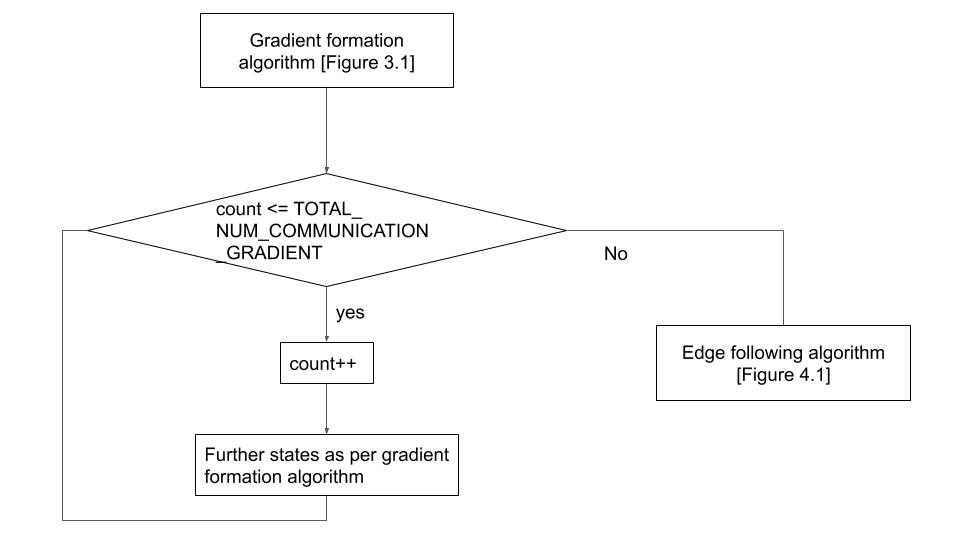
\includegraphics[scale=0.31]{images/flowchart-gradient&edge-following.jpg}}
	\caption{Integration of gradient formation and Edge following}
	\label{fig:Flowchart for integration of gradient formation and Edge following}
\end{figure}
\end{frame}

\begin{frame}
\frametitle{Demonstration}
\begin{figure}[H]
	\centering
	\fbox{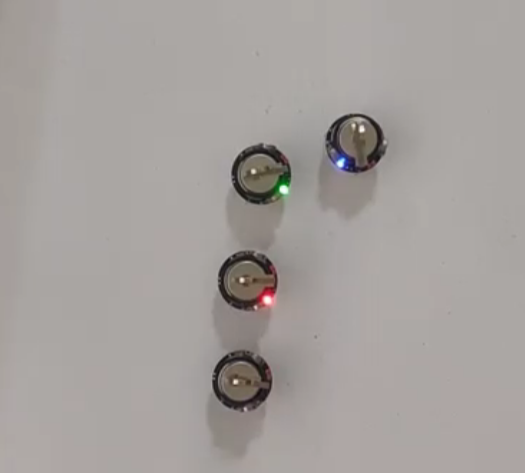
\includegraphics[width=2.4in]{images/gradient-edgefollowing.png}}
	\caption{\href{https://drive.google.com/file/d/1hssXnUnJvkTeVwVcXkR3x3gSFJD0FXtD/view}{Gradient formation and Edge following integration with \textit{TOTAL\_NUM\_COMMUNICATION\_GRADIENT=20} and \textit{TOTAL\_NUM\_COMMUNICATION = 15}}}
	\label{fig:Gradient formation and Edge following integration}
\end{figure}
\end{frame}




\begin{frame}
\frametitle{Conclusion}
\textbf{Future Scope}
\begin{itemize}
    \item Integration of work done by two batches
    \item Corner robot detection for a general shape
\end{itemize}
\vspace{0.2cm}
\newline
\textbf{Challenges}
\begin{itemize}
	\item Multiple reference kilobots
	\item Multiple kilobots with same unique ID
\end{itemize}
\end{frame}

\begin{frame}[allowframebreaks]{Reference}
\AtNextBibliography{\small}
\printbibliography
\end{frame}

\begin{frame}
  \begin{center}
  \textcolor{blue}{\Large THANK YOU!} 
  \end{center}
\end{frame}

\end{document}
